\chapter{Preliminary Testing}
\label{chap:\currfilebase}

\section{Preliminary Testing Setup}
\label{sec:preliminary_testing_setup}

The preliminary tests were conducted on the setup described in \autoref{chap:test_setup} but without the use of any tabbed specimens. In terms of setup preparation The CLC fixture of the setup did not provide any means to position the specimen inside the fixture with good repeatably. However the off-axis angle of the fibre direction was the main parameter that has been exposed during experiments. Hence its accuracy and repeatability was important for reliable test results. For this reason a positioning device was 3D-printed from PLA to target those issues. When assembling the fixture and specimen the positioning device is used as shown in \autoref{fig:fixture_positioner}.

\begin{figure}[!ht]
    \centering
    \begin{subfigure}[t]{\dimexpr(\distTextWidth-\distColSep)/2\relax}
        \centering
        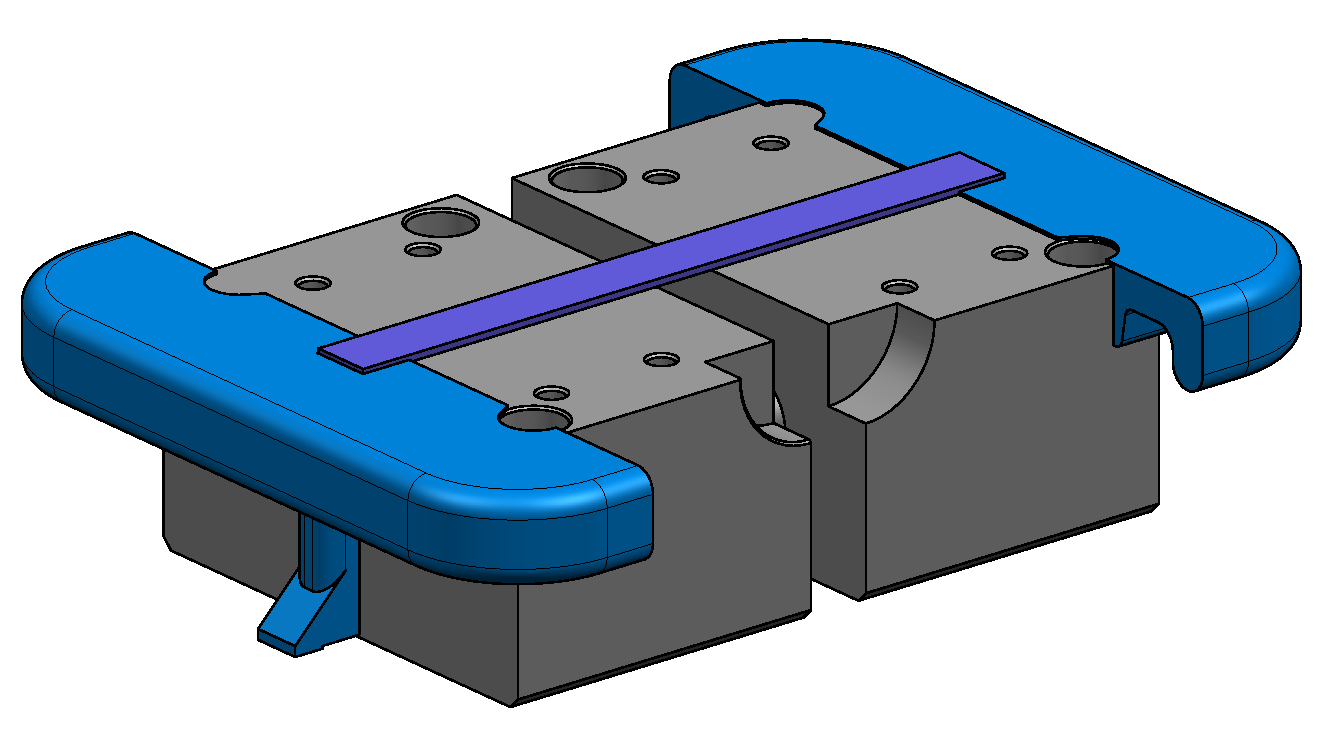
\includegraphics[scale=0.3]{\imgpath/\currfilebase/testfixture_positioner}
        \caption{untabbed specimen}
        \label{fig:fixture_positioner_untabbed}
    \end{subfigure}%
    \hfill
    \begin{subfigure}[t]{\dimexpr(\distTextWidth-\distColSep)/2\relax}
        \centering
        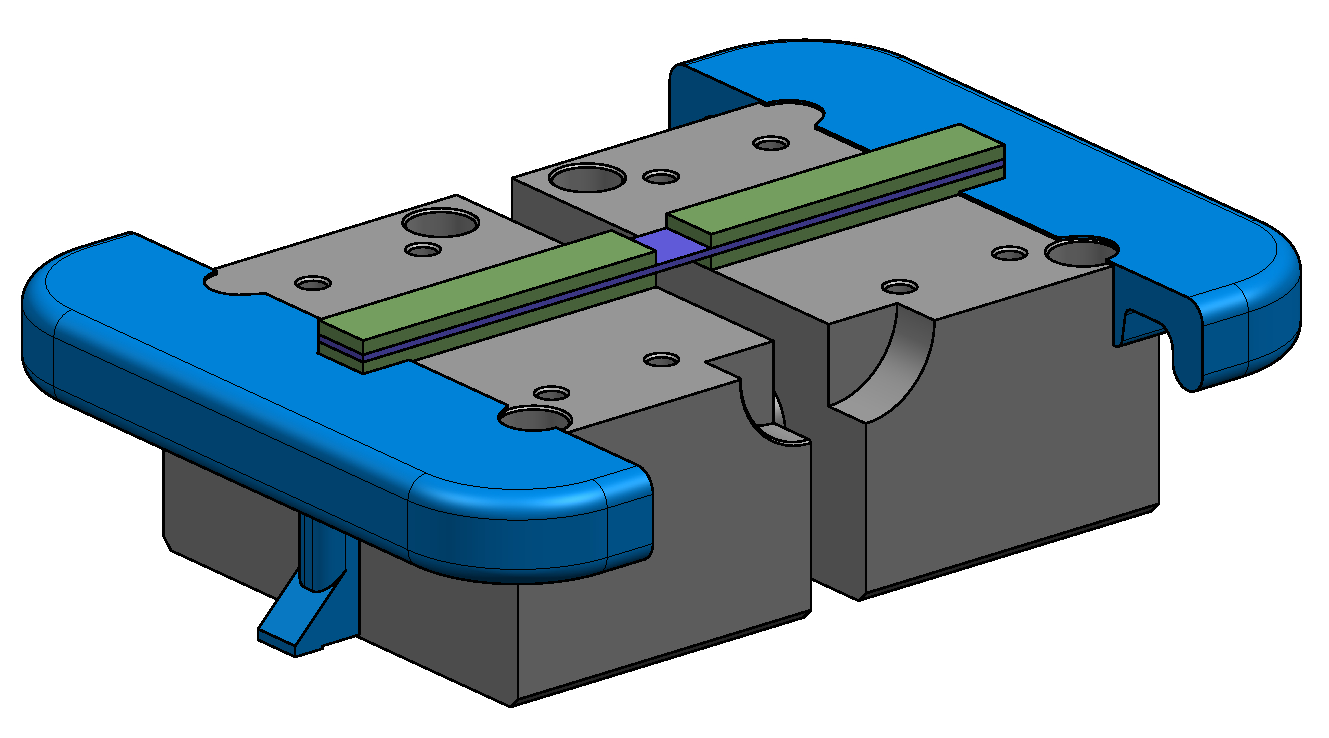
\includegraphics[scale=0.3]{\imgpath/\currfilebase/testfixture_positioner_tabbed}
        \caption{tabbed specimen}
        \label{fig:fixture_positioner_tabbed}
    \end{subfigure}
    \caption{3D-printed fixture positioner with specimen in violet, tabs in green, lower half of fixture in grey and fixture positioner in blue}
    \label{fig:fixture_positioner}
\end{figure}

\section{Preliminary Testing Results}
\label{sec:preliminary_testing_results}

In the preliminary testing specimens with off-axis below $\SI{20}{\degree}$ were prone to fail inside the fixture. This is an undesired use case since the CCD camera setup does not record the failure propagation. According to the fixture standard \cite{D6641standard} this is a common for unidirectional lamina and can be counteracted by tabbing the specimens.

The torque of the clamping skrews of the test fixture had a significant impact on the absolute compressive stress at failure. To counteract this variance the clamping skrews were fastened with a torque wrench, using the limit of $\SI{5}{\newton\meter}$ for most experiments.

\section{Tabbing Process}
\label{sec:tabbing_process}

Tabbed specimens were to be positioned by the same positioning device as untabbed ones, see \autoref{fig:fixture_positioner_tabbed}. Thus the tabbing process had to fulfill a high accuracy, so that the off-axis angle was reached with an equally good repeatably. Hence a 3D-printed tab positioner was used for aligning tabs and specimen during the adhesive bonding. The parts were assembled on pins as shown in \autoref{fig:tab_fixture_ass}.

\begin{figure}[!ht]
    \centering
    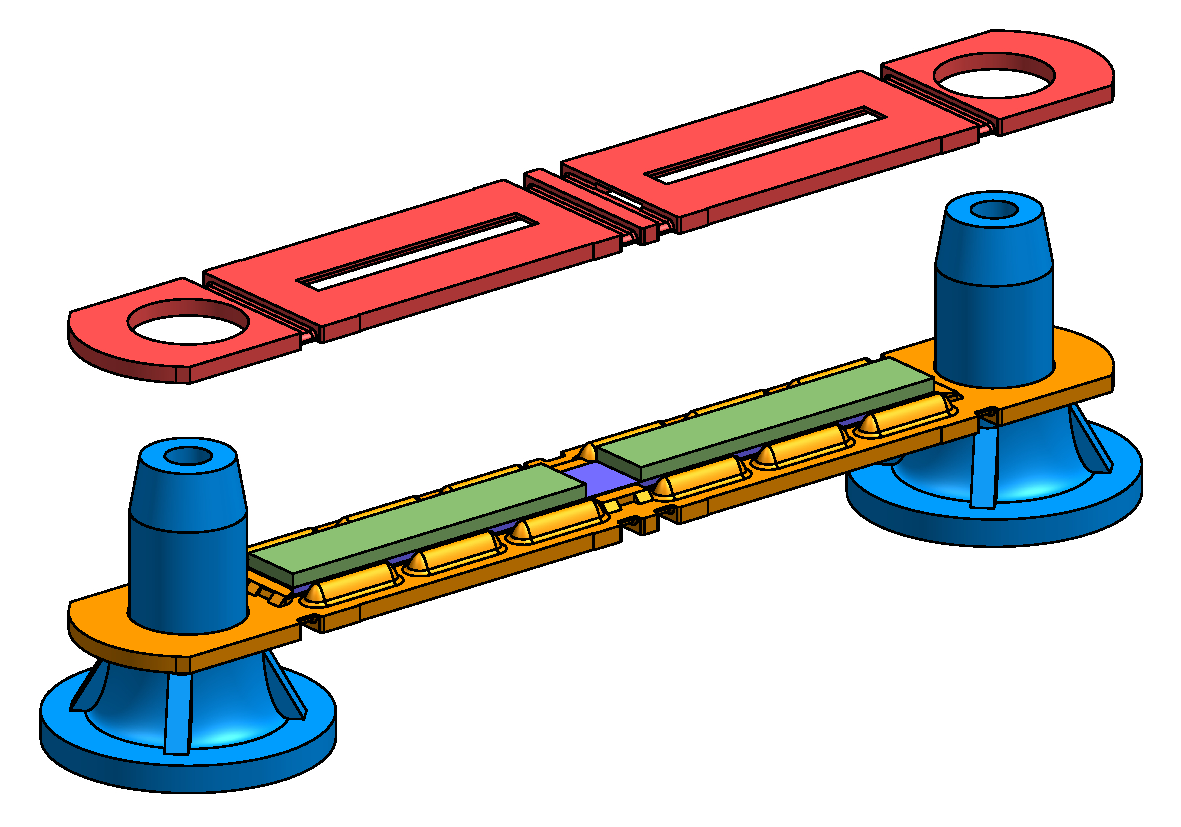
\includegraphics[scale=0.6]{\imgpath/\currfilebase/tab_fixture}
    \caption{Tabbing fixture assembly}
    \label{fig:tab_fixture_ass}
\end{figure}